\documentclass{standalone}
\usepackage{tikz}
\begin{document}
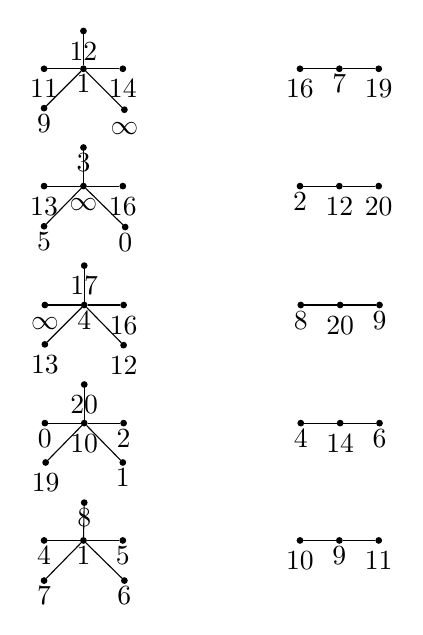
\begin{tikzpicture}[every node/.style={draw, circle, fill=black, minimum size=2pt, inner sep=0pt}]
\node[fill=black, label=below:{\color{black}$11$}] (G1N11) at (3.99,7.00) {};
\node[fill=black, label=below:{\color{black}$1$}] (G1N1) at (4.49,7.00) {};
\node[fill=black, label=below:{\color{black}$14$}] (G1N14) at (4.99,7.00) {};
\node[fill=black, label=below:{\color{black}$\infty$}] (G1Ninf) at (5.01,6.48) {};
\node[fill=black, label=below:{\color{black}$9$}] (G1N9) at (3.99,6.50) {};
\node[fill=black, label=below:{\color{black}$12$}] (G1N12) at (4.49,7.48) {};
\node[fill=black, label=below:{\color{black}$16$}] (G1N16) at (7.24,7.00) {};
\node[fill=black, label=below:{\color{black}$7$}] (G1N7) at (7.74,7.00) {};
\node[fill=black, label=below:{\color{black}$19$}] (G1N19) at (8.24,7.00) {};
\draw (G1N1) -- (G1N11);
\draw (G1N1) -- (G1N14);
\draw (G1N1) -- (G1Ninf);
\draw (G1N1) -- (G1N9);
\draw (G1N1) -- (G1N12);
\draw (G1N19) -- (G1N7);
\draw (G1N7) -- (G1N16);
\node[fill=black, label=below:{\color{black}$13$}] (G2N13) at (3.99,5.51) {};
\node[fill=black, label=below:{\color{black}$\infty$}] (G2Ninf) at (4.49,5.51) {};
\node[fill=black, label=below:{\color{black}$16$}] (G2N16) at (4.99,5.51) {};
\node[fill=black, label=below:{\color{black}$0$}] (G2N0) at (5.02,4.99) {};
\node[fill=black, label=below:{\color{black}$5$}] (G2N5) at (3.99,5.00) {};
\node[fill=black, label=below:{\color{black}$3$}] (G2N3) at (4.49,6.00) {};
\node[fill=black, label=below:{\color{black}$2$}] (G2N2) at (7.24,5.51) {};
\node[fill=black, label=below:{\color{black}$12$}] (G2N12) at (7.74,5.51) {};
\node[fill=black, label=below:{\color{black}$20$}] (G2N20) at (8.24,5.51) {};
\draw (G2Ninf) -- (G2N13);
\draw (G2Ninf) -- (G2N16);
\draw (G2Ninf) -- (G2N0);
\draw (G2Ninf) -- (G2N5);
\draw (G2Ninf) -- (G2N3);
\draw (G2N20) -- (G2N12);
\draw (G2N12) -- (G2N2);
\node[fill=black, label=below:{\color{black}$\infty$}] (G3Ninf) at (4.00,4.00) {};
\node[fill=black, label=below:{\color{black}$4$}] (G3N4) at (4.50,4.00) {};
\node[fill=black, label=below:{\color{black}$16$}] (G3N16) at (5.00,4.00) {};
\node[fill=black, label=below:{\color{black}$12$}] (G3N12) at (5.00,3.49) {};
\node[fill=black, label=below:{\color{black}$13$}] (G3N13) at (4.00,3.50) {};
\node[fill=black, label=below:{\color{black}$17$}] (G3N17) at (4.50,4.50) {};
\node[fill=black, label=below:{\color{black}$8$}] (G3N8) at (7.25,4.00) {};
\node[fill=black, label=below:{\color{black}$20$}] (G3N20) at (7.75,4.00) {};
\node[fill=black, label=below:{\color{black}$9$}] (G3N9) at (8.25,4.00) {};
\draw (G3N4) -- (G3Ninf);
\draw (G3N4) -- (G3N16);
\draw (G3N4) -- (G3N12);
\draw (G3N4) -- (G3N13);
\draw (G3N4) -- (G3N17);
\draw (G3N9) -- (G3N20);
\draw (G3N20) -- (G3N8);
\node[fill=black, label=below:{\color{black}$0$}] (G4N0) at (4.00,2.50) {};
\node[fill=black, label=below:{\color{black}$10$}] (G4N10) at (4.50,2.50) {};
\node[fill=black, label=below:{\color{black}$2$}] (G4N2) at (5.00,2.50) {};
\node[fill=black, label=below:{\color{black}$1$}] (G4N1) at (4.99,2.00) {};
\node[fill=black, label=below:{\color{black}$19$}] (G4N19) at (4.01,2.00) {};
\node[fill=black, label=below:{\color{black}$20$}] (G4N20) at (4.50,2.99) {};
\node[fill=black, label=below:{\color{black}$4$}] (G4N4) at (7.25,2.50) {};
\node[fill=black, label=below:{\color{black}$14$}] (G4N14) at (7.75,2.50) {};
\node[fill=black, label=below:{\color{black}$6$}] (G4N6) at (8.25,2.50) {};
\draw (G4N10) -- (G4N0);
\draw (G4N10) -- (G4N2);
\draw (G4N10) -- (G4N1);
\draw (G4N10) -- (G4N19);
\draw (G4N10) -- (G4N20);
\draw (G4N6) -- (G4N14);
\draw (G4N14) -- (G4N4);
\node[fill=black, label=below:{\color{black}$4$}] (G5N4) at (3.99,1.01) {};
\node[fill=black, label=below:{\color{black}$1$}] (G5N1) at (4.49,1.01) {};
\node[fill=black, label=below:{\color{black}$5$}] (G5N5) at (4.99,1.01) {};
\node[fill=black, label=below:{\color{black}$6$}] (G5N6) at (5.01,0.50) {};
\node[fill=black, label=below:{\color{black}$7$}] (G5N7) at (3.99,0.50) {};
\node[fill=black, label=below:{\color{black}$8$}] (G5N8) at (4.50,1.49) {};
\node[fill=black, label=below:{\color{black}$10$}] (G5N10) at (7.24,1.01) {};
\node[fill=black, label=below:{\color{black}$9$}] (G5N9) at (7.74,1.01) {};
\node[fill=black, label=below:{\color{black}$11$}] (G5N11) at (8.24,1.01) {};
\draw (G5N1) -- (G5N4);
\draw (G5N1) -- (G5N5);
\draw (G5N1) -- (G5N6);
\draw (G5N1) -- (G5N7);
\draw (G5N1) -- (G5N8);
\draw (G5N10) -- (G5N9);
\draw (G5N9) -- (G5N11);
\end{tikzpicture}
\end{document}
